\subsection{Versão Híbrida: MPI + OpenMP em Dois Níveis}
\label{sec:hibrido}

A versão híbrida une os dois modelos hierarquicamente: no nível macro, o MPI gerencia o pipeline de \textit{chunks} entre processos; no nível micro, o OpenMP paraleliza o interior de cada \textit{chunk} em tarefas 2D. 

\begin{figure}[H]
\centering
\begin{minipage}[b]{0.45\textwidth}
\centering
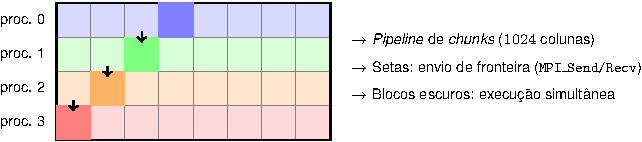
\includegraphics[height=2.2cm]{images/mpi_pipeline.pdf}
\caption*{(a) \textit{Pipeline} de \textit{chunks} no MPI.}
\end{minipage}\hfill
\begin{minipage}[b]{0.52\textwidth}
\centering
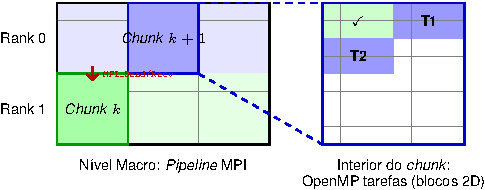
\includegraphics[height=2.2cm]{images/hibrido_arquitetura.pdf}
\caption*{(b) Híbrido: blocos OpenMP no \textit{chunk}.}
\end{minipage}
\caption{Modelos de execução distribuída e híbrida: (a) pipeline MPI; (b) tarefas OpenMP no \textit{chunk}.}
\label{fig:mpi_hibrido_pipeline}
\end{figure}

A comunicação usa \texttt{MPI\_THREAD\_FUNNELED}, assegurando que apenas a thread principal execute chamadas MPI fora de regiões paralelas. Como a largura do \textit{chunk} é $1024$ e o bloco OpenMP é $512$, há no máximo $\lceil 1024/512 \rceil = 2$ blocos na anti-diagonal por \textit{chunk}, limitando o paralelismo útil a 2 threads/processo e explicando a saturação do híbrido com mais threads.
